%% Setup und Metadaten einfügen
\documentclass[twocolumn]{scrartcl}

\usepackage[utf8]{inputenc}
\usepackage[ngerman]{babel}
\usepackage[T1]{fontenc}
\usepackage{graphicx}
\usepackage{listings}
\usepackage{xcolor}
\usepackage[german=guillemets]{csquotes}		%% Zitieren
\usepackage{amsmath}							%% Mathe
\usepackage{mathtools}
\DeclarePairedDelimiter\abs{\lvert}{\rvert}
\usepackage[hidelinks]{hyperref}				%% Ausblenden der Boxen um Referenzen
\usepackage{lmodern}							%% Schriftart
%%\usepackage[headsepline]{scrlayer-scrpage}		%% Individuelle Kopf- und Fußzeile
\usepackage[absolute]{textpos}
\usepackage{pdfpages}
\usepackage[a4paper, left=2cm, right=2cm, top=3cm, bottom=3cm]{geometry} %% Aändern der Seitenränder
\usepackage{trfsigns}


\KOMAoptions
{
	fontsize=9pt,								%% Schriftgröße
	parskip=half,								%% Absatz haben Einzug(off) oder Abstand(full, half)
	headings=normal								%% Größe der Überschriften
}


%% Codeumgebung settings
% color
\definecolor{codegray}{rgb}{0.9, 0.9, 0.9}

%%Listing setup
\lstset{
	backgroundcolor=\color{codegray},
	captionpos=b,
	breaklines=true,
}

\lstdefinestyle{customc}{
	language=C,
	breaklines=true,
	frame=L,
	basicstyle=\footnotesize\ttfamily,
	commentstyle=\itshape\color{green!60!black},
	keywordstyle=\bfseries\color{blue},
	identifierstyle=\color{purple!80!black},
	stringstyle=\color{red},
	xleftmargin=\parindent,
	showstringspaces=false,
	morekeywords={uint8_t, int8_t, uint32_t},
}



%% Quellenverzeichnis (Biblatex mit biber)
\usepackage{csquotes}
\usepackage[backend=biber, style=ieee]{biblatex}
\addbibresource{content/bib/lit.bib}



%%% Einstellungen für Kopf- und Fußzeile
%\automark[section]{section}
%\clearpairofpagestyles
%\ihead{\headmark}
%\chead{}
%\ohead{\pagemark}						%% Include setup file
\newcommand*{\titel}{Zusammenfassung Information Theory and Coding}
\newcommand*{\autor}{Markus Velm}

\hypersetup
{
	pdftitle=\titel
	pdfauthor=\autor
}
						%% Include meta data



%%%%%%%%%%%%%%%%
\begin{document}
%%%%%%%%%%%%%%%%
	\pagenumbering{Roman}
	
	%% Titelseite & Inhaltsverzeichnis
	\begin{titlepage}
		
		\begingroup
			\centering
            \fontsize{18pt}{22pt}\selectfont
            {\bfseries \titel\par}
        \endgroup		
		
		\begingroup
			\centering
            \fontsize{12pt}{22pt}\selectfont
            {\bfseries \autor\par}
        \endgroup
		
		\tableofcontents
	\end{titlepage}
	
	\newpage
	
	\clearpage
	
	\fontsize{9pt}{9pt}\selectfont
	
	\pagenumbering{arabic}
	
	%% Abschnitte
	
	\section{Einleitung}

\subsection{Informationstheorie}

Bit: binary unit $\rightarrow$ Einheit für Information

bit: binary digit $\rightarrow$ bit als binäres Symbol

\textbf{Informationgehalt} 

je unwahrscheinlicher ein Symbol $x$ auftritt, desto mehr Information enhält es:

$\displaystyle{
    I(x) = ld\left( \frac{1}{P(x)} \right) = -ld(P(x))
}$

$P$: Wahrscheinlichkeit eines Symbols\\
$I$: Informationsgehalt $[I] = Bit$

\textbf{Entropie}

gemittelter Informationsgehalt einer Quelle $X$:

$\displaystyle{
    H(X) = \sum_{i} P(x_i) \cdot I(x_i) = - \sum_{i} P(x_i) \cdot ld(P(x_i))
}$

$H$: Entropie $[H] = Bit/Symbol$

\textbf{Entscheidungsgehalt}

Entropie wird maximal, wenn alle Symbole gleichwahrscheinlich sind
$\rightarrow$ Entscheidungsgehalt

$\displaystyle{
    H_0 = ld(N)
}$

$H_0$: Entscheidungsgehalt $[H_0] = Bit/Symbol$\\
$N$: Anzahl der Symbole eines Alphabets

\textbf{Redundanz}

$\displaystyle{
    R = H_0 - H
}$

$\displaystyle{
    r = \frac{R}{H_0}
}$

$R$: Redundanz $[R] = Bit/Symbol$\\
$r$: relative Redundanz

%%//TODO: mittlere Laenge Code

\subsection{Quellcodierung}

\subsubsection{Huffman-Code}

ist \textbf{Präfixcode:} ein Codewort ist niemals Anfang eines anderen Codewortes

Codebaum aufbauen:
\begin{enumerate}
    \item Ordne die Symbole nach Auftrittswahrscheinlichkeit
    \item Fasse Symbole mit niedrigster Wahrscheinlichkeit zu einem Symbol zusammen und addiere die Wahrscheinlichkeiten
    \item Wiederhole bis nur ein Symbol übrig bleibt
\end{enumerate}

Beschrifte die Pfade mit 1 und 0\\
$\rightarrow$ Codewort ergibt sich, indem man von Wurzel bis zum Blatt geht

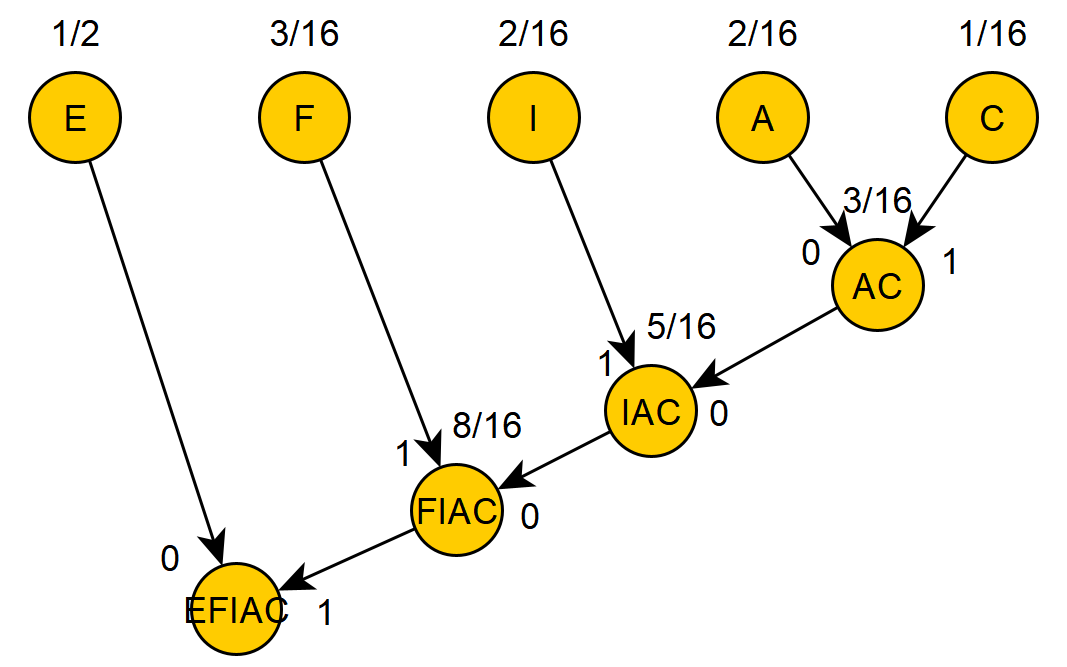
\includegraphics[width=6cm]{img/huffman.PNG}

\underline{Hinweis}: Beschriftung der 0; 1 theoretisch egal aber für Überprüfung mit Onlinerechnern
sollte konsistent der Pfad mit der geringeren und höheren Wahrscheinlichkeit gleich beschriftet
werden

\subsubsection{Arithmetische Codierung}

Codierung eines Wortes (oder Textes) durch Zahl

Endezeichen notwendig, da keine natürliche Terminierung des Codes

%//TODO arithmetische Codierung

\subsection{Kanalmodell}

\subsubsection{Binärkanal}

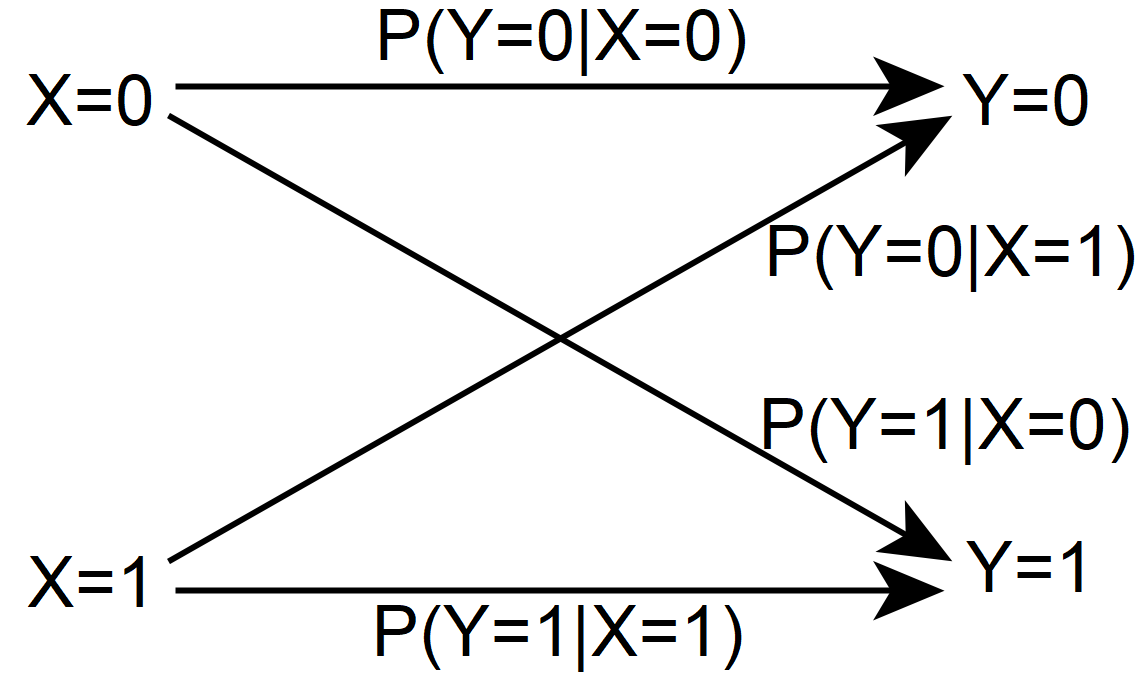
\includegraphics[width=4cm]{img/kanalmodell.PNG}

$P(Y|X)$: \frqq Wahrscheinlichkeit für Y, wenn X gesendet wurde\flqq (a-priori-Wahrscheinlichkeit)

$P(X|Y)$: \frqq Wahrscheinlichkeit für X, wenn Y empfangen wurde\flqq (a-posteriori-Wahrscheinlichkeit)

\textbf{Unxymmetrisch}: Fehlerwahrscheinlichkeit für \frqq 0\flqq{} und \frqq 1\flqq{} unterschiedlich

$\displaystyle{
    \begin{pmatrix}
        P(Y|X)    
    \end{pmatrix}
    =
    \begin{pmatrix}
        P(0|0) & P(0|1)\\
        P(1|0) & P(1|1)
    \end{pmatrix}
}$

\textbf{Symmetrisch}: Bitfehlerwahrscheinlichkeit $P_e$ für \frqq 0\flqq{} und \frqq 1\flqq{} gleich

$\displaystyle{
    \begin{pmatrix}
        P(Y|X)    
    \end{pmatrix}
    =
    \begin{pmatrix}
        P(0|0) & P(0|1)\\
        P(1|0) & P(1|1)
    \end{pmatrix}
    =
    \begin{pmatrix}
        1-P_e & P_e\\
        P_e & 1-P_e
    \end{pmatrix}
}$

\subsubsection{Bedingte Entropie}

$\displaystyle{
    H(Y|X) = - \sum_{j} \sum_{i} P(x_i, y_i)\,ld(P(y_i|x_i))
}$\;\; \textbf{Irrelevanz}

$\displaystyle{
    H(X|Y) = - \sum_{j} \sum_{i} P(x_i, y_i)\,ld(P(x_i|y_i))
}$\;\; \textbf{Äquivokation}

$H(Y|X)$: \textbf{Irrelevanz (Fehlinformation)}, mittlere Unsicherheit über empfangene Symbole, wenn Sendesymbole bekannt\\
$H(X|Y)$: \textbf{Äquivokation (Informationsverlust)}, mittlere Unsicherheit über gesendete Symbole, wenn Empfangssymbole bekannt

\subsubsection{Entropiemodell}

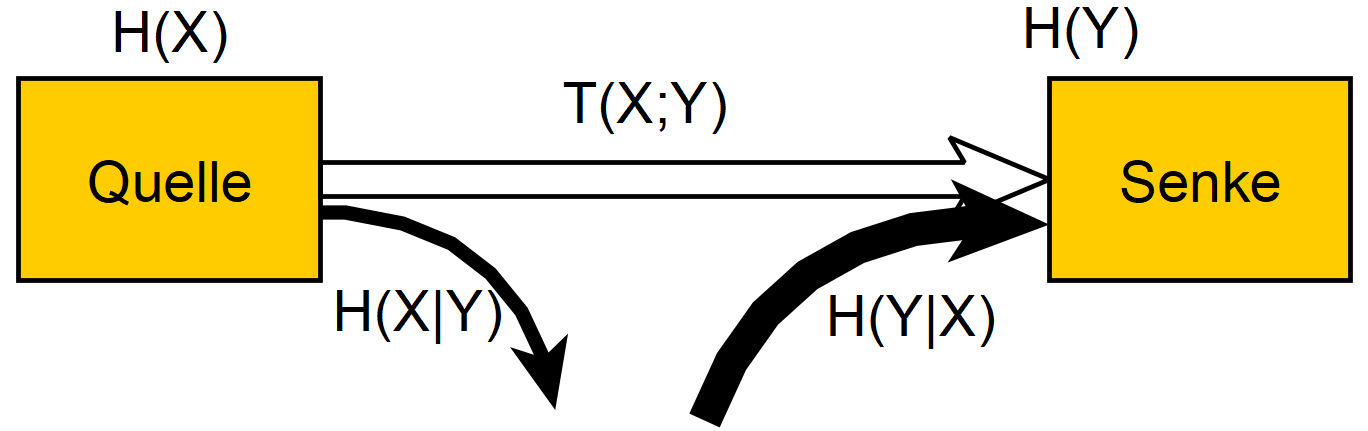
\includegraphics[width=7cm]{img/entropiemodell.PNG}

für Empfänger ist $H(Y)$ (also der Ausgang des Kanals) eine neue Quelle, allerdings mit zusätzlicher Fehlinformation

Die Transinformation ist dann die Entropie des Kanals minus der Fehlinformation

$\displaystyle{
    T(X;Y) = H(Y) - \underbrace{H(Y|X)}_{\text{Fehlinformation}}
}$

oder die Entropie der Quelle minus des Informationsverlusts

$\displaystyle{
    T(X;Y) = H(X) - \underbrace{H(X|Y)}_{\text{Informationsverlust}}
}$

Fehlinformation größer als Informationsverlust (außer es passieren keine Fehler,
oder die Entropie der Quelle ist maximal, dann $H(X|Y) = H(Y|X)$)

$\hookrightarrow$ Entropie am Ausgang des Kanals größer als die der Quelle (außer es passieren keine Fehler, oder die
Entropie der Quelle ist maximal, dann $H(X) = H(Y) = 1$)

\subsection{Kanalkapazität}

Die Kanalkapazität ist das Maximum an Information, welche über den Kanal geht

$\displaystyle{
    C = \max(T(X;Y)) = \max(H(X) - H(X|Y))
}$

$\displaystyle{
\;\;\;= \max(H(Y) - H(Y|X))
}$

$\displaystyle{
\;\;\;= 1 - H(X|Y) = 1 - H(Y|X)
}$

für binären, symmetrischen Kanal:

$\displaystyle{
    H(Y|X) = -p \cdot ld(p) - (1 - p) \cdot ld(1 - p)
}$

$\displaystyle{
    C = 1 + p \cdot ld(p) + (1 - p) \cdot ld(1 - p)
}$

$\displaystyle{
    C_S = C \cdot R_S
}$

$p$: Bitfehlerwahrscheinlichkeit\\
$C$: Kanalkapazität in Information/Symbol $[C] = Bit/Symbol$\\
$C_S$: Kanalkapazität in Information/Zeit $[C_S] = Bit/s$\\
$R_S$: Symbolrate $[R_S] = Symbol/s$

\textbf{Informationsfluss}

$\displaystyle{
    H_S = H \cdot R_S
}$

$H_S$: Informationsfluss in Information/Zeit $[H_S] = Bit/s$\\
$H$: Informationsgehalt pro Symbol $[H] = Bit/Symbol$\\
$R_S$: Symbolrate $[R_S] = Symbol/s$

\subsection{Shannon-Theoreme}

\subsubsection{Erster Satz von Shannon}

Quellcodierung

Ist ein Informationsfluss von $H_S$ gewünscht, welcher kleiner als die Kanalkapazität $C_S$ ist,
ist es möglich einen Code zu finden, sodass der Informationsfluss übertragen werden kann

\subsubsection{Zweiter Satz von Shannon}

Kanalcodierung

Ist der die gewünschte Datenfluss $R_S$ ($[R_S] = Symbol/s = bit/s$) kleiner als die Kanalkapazität $C_S$, dann
gibt es einen Code, sodass die Fehlerwahrscheinlichkeit beliebig klein wird

\subsubsection{Shannon-Hartley}

Kanalkapazität abhängig vom SNR

$\displaystyle{
    C_S = W \cdot ld\left( 1 + \frac{S}{N} \right)
}$

$C_S$: Kanalkapazität in Information/Zeit $[C_S] = Bit/s$\\
$W$: Bandbreite $[W] = Hz$\\
$S$: Signalleistung\\
$N$: Rauschleistung

\textbf{Bandbreiteneffizienz}

Wird mit $R_S = C_S$ übertragen, kann die Bandbreiteneffizienz bestimmt werden

$\displaystyle{
    \frac{R_S}{W} = ld\left( 1 + \frac{S}{N} \right)
}$

$\displaystyle{
    S = \frac{E_b}{T_b} = E_b \cdot R_S
}$\;\;\;\;\;\;\;\;\;\;
$\displaystyle{
    N = N_0 \cdot W
}$

$\displaystyle{
    \frac{S}{N} = \frac{E_b \cdot R_S}{N_0 \cdot W}
}$

$\hookrightarrow$ damit S/N \underline{und} Bandbreiteneffizienz abhängig von $W$

Ist eine Bandbreiteneffizienz gewünscht, kann das erfolderliche S/N ausgerechnet werden

$\displaystyle{
    \frac{E_b}{N_0} = \frac{W}{R_S} ld \left( 2^{\frac{R_S}{W}} - 1 \right)
}$

$\displaystyle{
    \frac{E_b}{N_0}_{min} = -1,6\,dB
}$

$\frac{R_S}{W}$: Bandbreiteneffizienz $[\frac{R_S}{W}] = \left(\frac{bit/s}{Hz}\right)$\\
$E_b$: Energie die für die Übertragung von 1 bit aufgewendet wird $[E_b] = J = Ws = W/Hz$\\
$T_b$: Zeitdauer eines bits $[T_b] = s = 1/Hz$

\section{Blockcodes}

Code beschrieben durch $C(n, k, d)$

$n$: Länge Codewort\\
$k$: Länge Informationswort\\
$d$: Mindestabstand

Coderate: 
$\displaystyle{
    CR = \frac{k}{n}
}$

\subsection{Generelles}

\textbf{Generatormatrix}

Erzeugung eines Codewortes über Multiplikation eines Informationsvektors

$\displaystyle{
    \vec{c} = i \cdot G
}$

$c$: Codewort\\
$i$: Informationswort\\
$G$: Generatormatrix

\textbf{Prüfmatrix}

$\displaystyle{
    H \vec{c}^T = 0
}$

$\displaystyle{
    H \cdot G^T
}$

$H$: Prüfmatrix

\textbf{Syndrom}

wenn Empfangswort $r$ fehlerhaft ist (und nicht zum Coderaum gehört) dann ist das Produkt aus
Prüfmatrix und Empfangswort das \textit{Syndrom} und nicht mehr 0

$\displaystyle{
    H \vec{r}^T = H (\vec{c} + \vec{f})^T = H \vec{f}^T = \vec{s} \neq 0
}$

\textbf{Systematische Codes}

Systematischer Code: Einheitsmatrix $I$ ist Teil der Generatormatrix

$\displaystyle{
    G = [I | G']
}$

Bsp.: C(7, 4, 3): 
$\displaystyle{
    G =
    \begin{pmatrix}
        1 & 0 & 0 & 0 & 0 & 1 & 1\\
        0 & 1 & 0 & 0 & 1 & 0 & 1\\
        0 & 0 & 1 & 0 & 1 & 1 & 0\\
        0 & 0 & 0 & 1 & 1 & 1 & 1
    \end{pmatrix}
}$

\textbf{Lineare Codes}

Eigenschaften:
\begin{itemize}
    \item Mindestgewicht = Mindestabstand
    \item Codewort + anderes Codewort = wieder Codewort
    \item Nullwort ist teil des Codes
\end{itemize}

\textbf{Gewicht}

Gewicht eines Codewortes: Anzahl der von 0 verschiedenen Stellen

Mindestgewicht: Minimale Anzahl an Stellen, die von 0 verschieden sind

\textbf{Distanz/Abstand}

Hamming-Distanz: Anzahl verschiedener Stellen zweier Codewörter

Mindestdistanz: Mindestanzahl verschiedener Stellen zweier beliebiger Codewörter eines Codes

\textbf{Fehlerkorrektur/Fehlererkennung}

Anzahl der korrigierbaren Fehler $e$ bei gegebenem Abstand $d$

$\displaystyle{
    e = \Bigl\lfloor \frac{d - 1}{2} \Bigr\rfloor
}$

\underline{bei ungeradem $d$:}

es werden $d-1$ Fehler erkannt

\underline{bei geradem $d$:}

es werden alle ungeraden Anzahlen an Fehlern erkannt

\subsection{Fehlerwahrscheinlichkeit}

\textbf{Restblockfehlerwahrscheinlichkeit}

Wahrscheinlichkeit, dass von $n$ Symbolen beliebige $m$ falsch und die übrigen Symbole $n-m$ richtig sind:

$\displaystyle{
    \binom{n}{m} \cdot p^m \cdot (1 - p)^{n-m}
}$

\underline{für ungerades $d$:}

alle Fehler werden entweder korrigiert, oder nicht erkannt

Kann ein Code $e$ Fehler korrigieren, dann verbleibt eine Restblockfehlerwahrscheinlichkeit von:

$\displaystyle{
    P_{Block} = \sum_{m = e + 1}^{n} \binom{n}{m} \cdot p^m \cdot (1 - p)^{n-m}
}$

$\displaystyle{
    = 1 - \sum_{m=0}^{e} \binom{n}{m} \cdot p^m \cdot (1 - p)^{n-m}
}$

$p$: Fehlerwahrscheinlichkeit vor der Decodierung\\
$P_{Block}$: Wahrscheinlichkeit, für Symbolfehler im decodierten Block

\underline{für gerades $d$:}

alle ungeraden Fehler werden erkannt, da sie nicht in Korrekturkugeln liegen; können damit aber auch
nicht korrigiert werden

$\rightarrow$ für die Wahrscheinlichkeit, dass Fehler nicht erkannt werden, tragen also nur die geraden Fehleranzahlen, welche größer als $e$ sind, bei

$\displaystyle{
    P_{Block,erkennen} = \sum_{m=e+1}^{n} \binom{n}{2m} \cdot p^{2m} \cdot (1 - p)^{n-2m}
}$

$P_{Block}$ gleich wie bei gerader Anzahl

\textbf{Symbolfehlerwahrscheinlichkeit}

Block besteht aus $k$ Symbolen

Bei gegebener Restblockfehlerwahrscheinlichkeit, gibt es eine Symbolfehlerwahrscheinlichkeit von

$\displaystyle{
    P_{Symb} = P_{S|Block} \cdot P_{Block} = \frac{2^{k-1}}{2^k - 1} P_{Block}
}$

\subsection{Hamming-Codes}

immer $d=3$, damit immer $e=1$

$\displaystyle{
    n = 2^h - 1
}$

$\displaystyle{
    k = n - h
}$

\begin{tabular}{c|c c c}
    h & n & k & d\\
    \hline
    2 & 3 & 1 & 3\\
    3 & 7 & 4 & 3\\
    4 & 15 & 11 & 3\\
    5 & 31 & 26 & 3\\
    \vdots & \vdots & \vdots & \vdots
\end{tabular}

\textbf{Konstruktion}

\underline{1. Erstellung Prüfmatrix}

Spalten sind Dualdarstellung der Spaltennummer

$H_{n-k x n}$

Beispiel: C(7, 4, 3)

$\displaystyle{
    H_{3 x 7} = \begin{pmatrix}
        0 & 0 & 0 & 1 & 1 & 1 & 1\\
        0 & 1 & 1 & 0 & 0 & 1 & 1\\
        1 & 0 & 1 & 0 & 1 & 0 & 1
    \end{pmatrix}
}$

\underline{2. Spalten tauschen, sodass hinten Einheitsmatrix}

$H = [A_{n-k x k} | I_{n-k x n-k} ]$

Spalte 1 mit 7\\
2 mit 6\\
4 mit 5

$\displaystyle{
    \rightarrow H = \begin{pmatrix}
        1 & 1 & 0 & 1 & 1 & 0 & 0\\
        1 & 1 & 1 & 0 & 0 & 1 & 0\\
        1 & 0 & 1 & 1 & 0 & 0 & 1
    \end{pmatrix} = [ A_{3 x 4} | I_{3 x 3} ]
}$

\underline{3. Generatormatrix aufstellen}

$G_{k x n} = [I_{k x k} | -A^T_{k x n-k} ]$

$\displaystyle{
    G = \begin{pmatrix}
        1 & 0 & 0 & 0 & 1 & 1 & 1\\
        0 & 1 & 0 & 0 & 1 & 1 & 0\\
        0 & 0 & 1 & 0 & 0 & 1 & 1\\
        0 & 0 & 0 & 1 & 1 & 0 & 1
    \end{pmatrix}
}$

systematisch, da Informationswort zusammenhängend im Codewort steht

\underline{4. Rücktauschen der Spalten}

Spalte 1 mit 7\\
2 mit 6\\
4 mit 5

$\displaystyle{
    G = \begin{pmatrix}
        1 & 1 & 0 & 1 & 0 & 0 & 1\\
        0 & 1 & 0 & 1 & 0 & 1 & 0\\
        1 & 1 & 1 & 0 & 0 & 0 & 0\\
        1 & 0 & 0 & 1 & 1 & 0 & 0
    \end{pmatrix}
}$

quasi-systematisch, da Informationswort zwar im Codewort, aber nicht zusammenhängend

\textbf{Fehler und Syndrom}

Fehler gibt an, an welcher Stelle des Empfangsworts ein Fehler aufgetreten ist

Bsp.:

$\displaystyle{
    \vec{s} = \begin{pmatrix}
        0\\
        1\\
        1
    \end{pmatrix}
}$

$\rightarrow$ Fehler an Stelle $(011)_b = 3$ im Empfangswort

$\rightarrow$ da binärer Code, muss für Fehlerkorrektur das dritte bit nur invertiert werden

\section{Galois-Felder}
\label{sec:galois}

\subsection{Algebraische Strukturen}

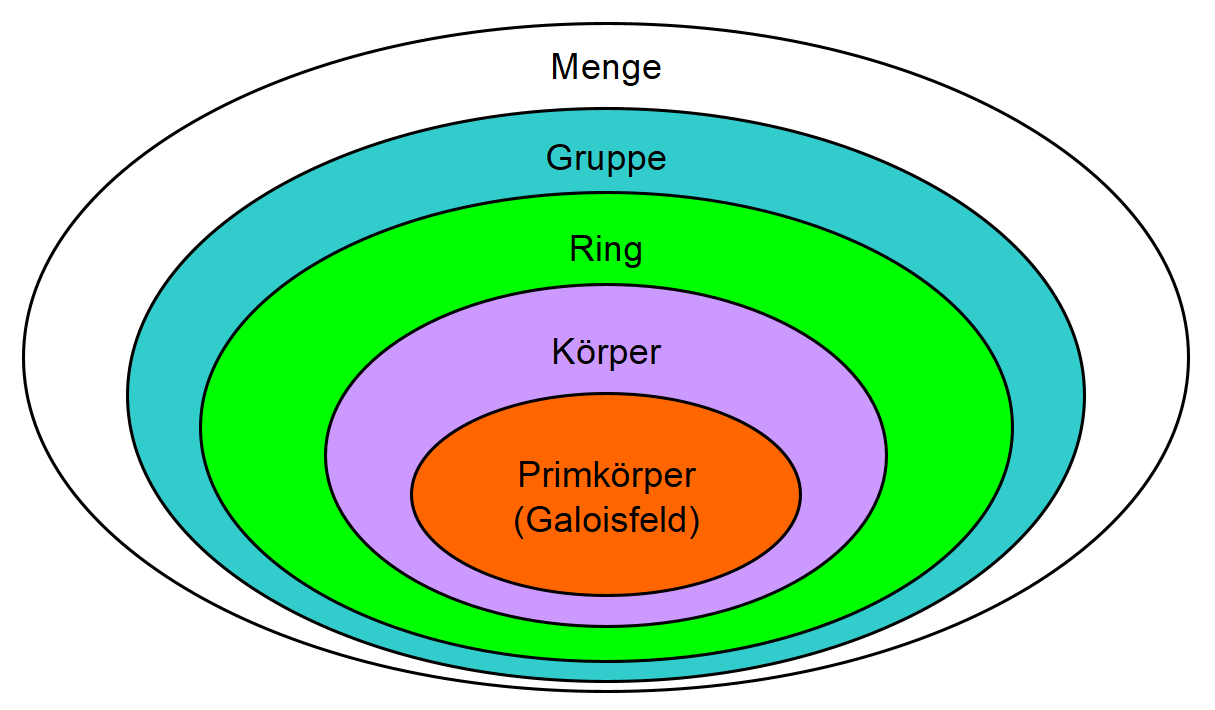
\includegraphics[width=8cm]{img/algebraische_strukturen.PNG}

\textbf{Menge}

Verbund von Elementen, welche keine Operationen beinhalten (Möbel können eine Menge sein, es kann aber nicht Tisch + Stuhl gerechnet werden)

\textbf{Halbgruppe}

Menge $A$ mit Verknüpfung \frqq +\flqq{} ist eine Halbgruppe, wenn
\begin{itemize}
    \item Abgeschlossenheit (+ zweier Elemente von $A$ ergibt wieder ein Element von $A$)
    \item Assoziativität (Reihenfolge der Operation mit + spielt keine Rolle, $a + (b + c) = (a + b) + c$)
    \item Existenz eines neutralen Elements (Element $a$ + neutrales Element $n$ ergibt wieder Element $a$)
\end{itemize}

\textbf{Gruppe}

Halbgruppe plus
\begin{itemize}
    \item Existenz eines additiven inversen Elements ($a + b = n$)
\end{itemize}

\textbf{Abelsche oder kommutative Gruppe}

Gruppe plus
\begin{itemize}
    \item Kommutativität (Reihenfolge der Operanden spielt keine Rolle, $a + b = b + a$)
\end{itemize}

\textbf{Ring}

abelsche Gruppe plus
\begin{itemize}
    \item Abgeschlossenheit bezüglich \frqq $\cdot$\flqq
    \item Assoziativität bezüglich \frqq $\cdot$\flqq
    \item Distributivität ($a \cdot (b + c) = a \cdot b + a \cdot c$)
\end{itemize}

\textbf{Körper}

Ring plus
\begin{itemize}
    \item Kommutativität bezüglich \frqq $\cdot$\flqq ($a \cdot b = b \cdot a$)
    \item Neutrales Element bezüglich \frqq $\cdot$\flqq
    \item Inverses Element bezüglich \frqq $\cdot$\flqq für jedes Element
\end{itemize}

\textbf{Primkörper/Galois-Feld}

Körper, indem Addition und Multiplikation $\mod p$ gerechnet wird ($p$ muss dabei eine Primzahl sein)\\
$\hookrightarrow GF(p)$

\subsection{Eigenschaften Galois-Felder}

\textbf{Primitives Element}

Element $\alpha$, welches durch ihre $p-1$ Potenzen alle Elemente (außer $0$) des $GF(p)$ erzeugt

Bsp. $GF(5), \alpha = 2$:

$2^0 = 1 \mod 5 = 1$\\
$2^1 = 2 \mod 5 = 2$\\
$2^2 = 4 \mod 5 = 4$\\
$ 2^3 = 8 \mod 5 = 3$

ab hier zykische Wiederholung:\\
$2^4 = 16 \mod 5 = 1$

\textbf{Polynome}

Folge an $n$ Zahlen im Galois-Feld wird als Polynom vom Grad $n-1$ geschrieben

$\displaystyle{
    \hookrightarrow \{ 1; 4; 3; 1 \} \rightarrow A(x) = 1x^3 + 4x^2 + 3x + 1
}$

Auswertung des Polynoms $A(x)$ an verschiedenen Stellen von $\alpha^i$ ergibt ihre Fouriertransformierte $a(x)$

$\displaystyle{
    a_i = A(\alpha^i)
}$

\textbf{Zyklische Faltung}

Polynommultiplikation im Galois-Feld $\rightarrow$ zyklische Faltung

Normale Faltung mit endlichen Signalen $\rightarrow$ endliches Faltungsergebnis

Zyklische Faltung: Signale sind periodisch, damit Faltungsergebnis ebenfalls periodisch (und damit unendlich lang)

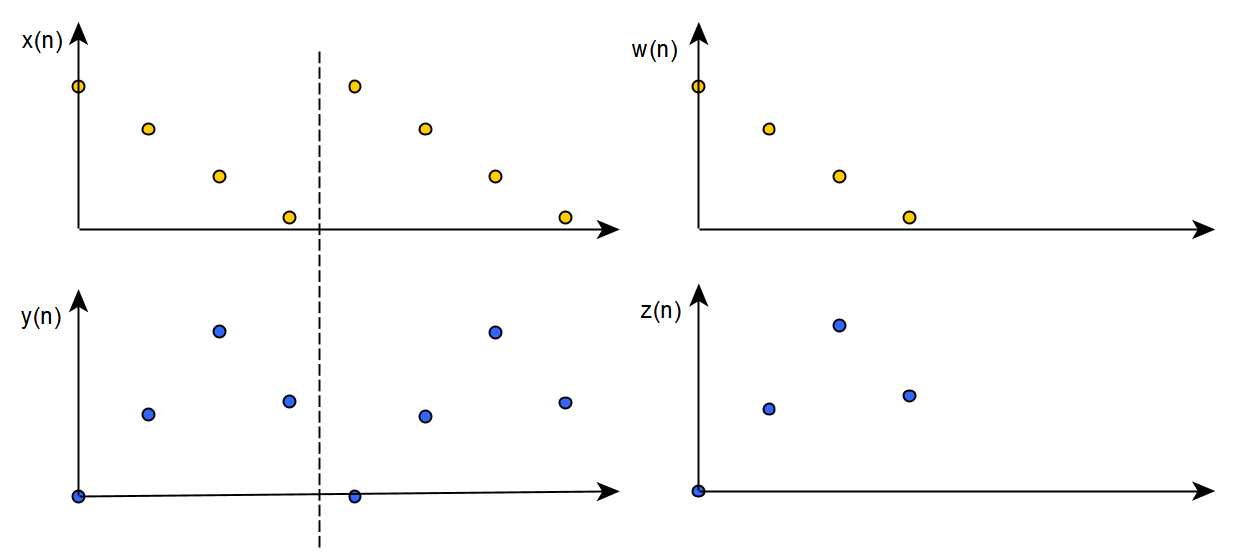
\includegraphics[width=8.7cm]{img/zykische_faltung.PNG}

links: zyklische Faltung \;\;\;\;\;\;\;\;\;\;\;\; rechts: normale Faltung

\section{Reed-Solomon-Code}

\subsection{Wunsch und Idee}

\textbf{Wunsch}

Konstruktion eines Codes mit vorgegebener Korrekturfähigkeit\\
$\rightarrow$ Vorgabe des Mindestabstandes $d$

$\displaystyle{
    e = \Bigl\lfloor \frac{d - 1}{2} \Bigr\rfloor
}$\\
$\displaystyle{
    d = 2e + 1
}$

bei linearem Code ist Mindestabstand = Mindestgewicht

$\rightarrow$ Codeworte haben mind. $d$ von 0 verschiedene Koeffizienten

d'Alembert: Polynom vom Grad $n$ hat $n$ komplexe (oder höchstens $n$ reelle) Nullstellen; auch
im Galois-Feld

\textbf{Idee}

Konstruktion des Informationswortes als Polynom $A(x)$ mit Grad $k-1$ (damit höchstens $k-1$ Nullstellen)

Im $GF(p)$ mit Ordnung $n = p-1$ kann man $A(x)$ an $n$ Stellen auswerten, danach wiederholen sich die Werte

$\rightarrow$ Auswertung des Polynoms für verschiedene $x$ (bzw. $\alpha^i$) ergeben die Koeffizienten $a_i$ des
Polynoms $a(x)$

$\displaystyle{
    a_i = A(\alpha^i) \qquad\qquad\qquad \text{\textbf{IDFT}}
}$

von diesen sind höchstens $k-1$ Null (weil $grad(A(x)) = k-1$)\\
von diesen sind also mind. $n - (k-1)$ von Null verschieden $\rightarrow$ Mindestgewicht $d$

$d = n - (k - 1) = n - k + 1$

Rücktransformation des Codeworts in Informationswort:

$\displaystyle{
    A_i = n^{-1} a(\alpha^{-i}) \qquad\qquad \text{\textbf{DFT}}
}$

\subsection{Codierung}

Verschiedene Möglichkeiten aus einem Informationswort ein Codewort zu generieren

\subsubsection{Generatorpolynom}
\label{subsubsec:gen-poly}

Erzeugt zusammenhängende Nullstellen im Codewort = Syndromstellen

$\displaystyle{
    g(x) = \prod_{i=k}^{n-1} \left(x - \alpha^{-i}\right)
}$

Syndromstellen beginnen hier bei $k$, es sind aber alle anderen Stellen möglich, solange sie zusammenhängen

$grad(g(x)) = d-1 = n-k$ = Anzahl Syndromstellen

$g(x)$: Generatorpolynom\\
$i(x)$: Informationspolynom

\subsubsection{Prüfpolynom}

Prüfpolynom:

$\displaystyle{
    h(x) = \prod_{i=0}^{k-1} \left(x - \alpha^{-i}\right)
}$

Produkt aus Generator- und Prüfpolynom ist 0

$\displaystyle{
    g(x) \cdot h(x) = 0
}$

und Produkt aus Codepolynom und Prüfpolynom ist 0

$\displaystyle{
    a(x) \cdot h(x) = 0
}$

genau da, wo $g(x)$ (oder $a(x)$) Nullstellen hat (also $G_i$ 0 ist) hat das Prüfpolynom $h(x)$ keine Nullstellen
(ist also $H_i$ nicht 0) und umgekehrt

\subsubsection{IDFT (nicht systematisch)}

$\displaystyle{
    a_i = A(\alpha^i)
}$

$A(x)$: Informationswort\\
$a_i$: Koeff. des Codewortes

\subsubsection{Polynommultiplikation (nicht systematisch)}

$\displaystyle{
    a_i = g(x) \cdot i(x)
}$

\subsubsection{Polynomdivision (systematisch)}

Informationswort ist Teil des Codewortes (an den hohen Potenzen)

$\displaystyle{
    a^*(x) = i_{k-1} x^{n-1} + i_{k-2} x^{n-2} + ... + i_1 x^{n-k+1} + i_0 x^{n-k}
}$

jedes Codewort muss durch Generatorpolynom teilbar sein $\rightarrow$ ist
für $a^*(x)$ i.A. nicht der Fall

$\displaystyle{
    \frac{a^*(x)}{g(x)} = b(x) + \frac{rest(a^*(x))}{g(x)}
}$\\
$\displaystyle{
    \rightarrow \frac{a^*(x) - rest\left(a^*(x)\right)}{g(x)} = b(x)
}$\\
$\displaystyle{
    a(x) = a^*(x) - rest\left(a^*(x)\right)
}$

$rest\left(a^*(x)\right)$: Divisionsrest

\subsubsection{Zyklischer Code}

Multiplikation eines Polynoms mit $x^i$ verschiebt Koeff. des Polynoms um $i$-Stellen

durch mod-Rechnung des Exponenten verschieben sich höhere Exponenten wieder an den Anfang des Polynoms

Bsp.:

$\displaystyle{
    x \cdot a(x) = x \cdot ( 2x^2 + x + 1 ) = 2x^3 + x^2 + x = x^2 + x + 2
}$

\subsection{Decodierung}

\textbf{Idee:}

Addition des Fehlerpolynoms $f(x)$ mit $t$ Koeffizienten (d.h. $t$ Fehler sind auf dem Kanal aufgetreten)
zum gesendeten Codewort $a(x)$

im Zeitbereich:

$\displaystyle{
    r(x) = a(x) + f(x)
}$

im Frequenzbereich:

$\displaystyle{
    R(x) = A(x) + F(x)
}$

gedanklich wird ein Polynom $c(x)$ aufgestellt, welches $t$ Nullen an den Fehlerstellen hat

Da die Koeffizienten von $c(x)$ die Auswertung ihrer Fouriertransformierten $C(x)$ ist, ist der Grad
von $C(x)$ $t$

Da $c(x)$ gerade dort 0 ist, wo $f(x)$ ungleich 0, ist das Produkt $f_i \cdot c_i$ immer 0 (Achtung, keine
Polynommultiplikation gemeint, sondern punktweise Multiplikation)

$\displaystyle{
    f_i \cdot c_i = 0
}$

wenn Zeitbereich = 0 $\rightarrow$ Frequenzbereich = 0

$\displaystyle{
    F(x) \cdot C(x) = 0
}$

Achtung: hier Polynommultiplikation/ Faltung/ Filterung gemeint\\
$\hookrightarrow$ Aufstellen der Schlüsselgleichungen

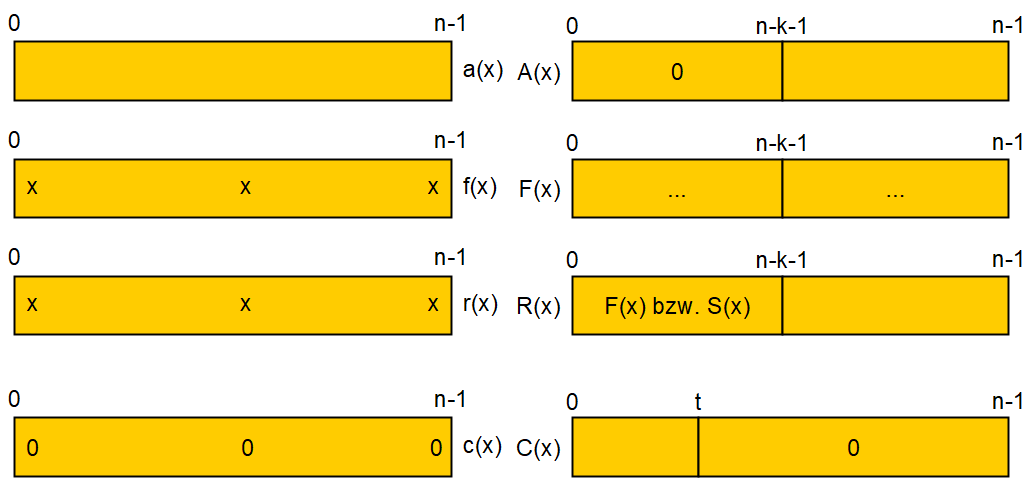
\includegraphics[width=8cm]{img/decod_rs.PNG}

\subsubsection{Vorgehen}

\begin{enumerate}
    \item Fouriertransformation des empfangenen Codewortes $r(x) \rightarrow R(x)$
    \item Auslesen der Koeff. des Syndrompolynoms ($S_0, ..., S_n$) aus $R(x)$ und Aufstellen des Syndrompolynoms
    \item Berechnung des $C(x)$ aus Schlüsselgleichungen oder euklidschem Algorithmus
    \item Berechnung der Fehlerstellen durch Nullstellensuche von $C(x)$
    \item Berechnung des Fehlerwertes über Schlüsselgleichungen oder Forney-Algorithmus
\end{enumerate}

\subsubsection{Schlüsselgleichungen}

beschreiben, dass Faltung von $C(x)$ und $F(x)$ Null ist (Achtung: zyklische Faltung, siehe \autoref{sec:galois})

$F_0$ bis $F_{n-k-1}$ (bzw. $F_{d-2}$) sind bekannt, da diese direkt an den Syndromstellen
von $R(x)$ stehen

Alle $C$-Koeff. sind unbekannt, außer $C_{t}$, dieser wird zu $1$ gesetzt

$\displaystyle{
    C_{t} = 1
}$

da Anzahl der Fehler ($t$) unbekannt ist, muss ausprobiert werden, welche \underline{minimale} Anzahl an Fehlern
die Schlüsselgleichungen widerspruchsfrei erfüllt

Lösen der Schlüsselgleichungen nach $C(x)$

$\hookrightarrow$ Nullstellensuche von $C(x)$ ergibt die Nullen des $c(x)$

$\hookrightarrow$ wenn Grad von $C(x)$ nicht mit Anzahl der Nullstellen übereinstimmt $\rightarrow$ Decodierversagen

Lösen der Schlüsselgleichungen nach $F(x)$

$\hookrightarrow f(x)$ aus Rücktransformation von $F(x)$

$\hookrightarrow f(x)$ von $r(x)$ abziehen, man erhält $a(x)$

$\displaystyle{
    a(x) = r(x) - f(x)
}$

%%// TODO: Schlüsselgleichungen aufstellen und eigentliche Schlüsselgleichungen

\subsubsection{Euklidscher Algorithmus}

Suche des ggT zweier Zahlen

Kann zur Lösung der Schlüsselgleichungen verwendet werden

Rest:

$\displaystyle{
    r_n = v_n a_n + w_n b_n
}$

Rekursionsformeln für $v_n$ und $w_n$:

$\displaystyle{
    v_n = v_{n-2} - q_n v_{n-1}
}$

$\displaystyle{
    w_n = w_{n-2} - q_n w_{n-1}
}$

$q_n$: Quotient des vorherigen Schrittes

Initialisierung:

$\displaystyle{
    v_{-1} = 1 \;\;\;\;\; v_0 = 0
}$\\
$\displaystyle{
    w_{-1} = 0 \;\;\;\;\; w_0 = 1
}$

Suche des $C(x)$ und damit den Fehlerstellen

Polynomdivision von $x^{d-1}$ und des Syndrompolynoms $S(x)$

$\displaystyle{
    x^{d-1} : S(x)
}$

Wenn Rest der Division im Grad nicht kleiner ist als die Anzahl der Fehler $e$, die maximal korrigiert
werden können $\rightarrow$ weiter: $S(x) : r_1(x)$

usw.

ist Grad des Restes kleiner als $e$ $\rightarrow$ Berechnung des $C(x)$ und des $T(x)$

$\hookrightarrow C(x) = w_n$

$\hookrightarrow T(x) = -r_n$

\subsubsection{Forney-Algorithmus}

Fehlerstellenberechnung durch Nullstellensuche in $C(x)$

$\displaystyle{
    c_i = C(\alpha^i)
}$

Fehlerwertberechnung aus gegebenem $C(x)$ und $T(x)$

$\displaystyle{
    f_i = x^q \cdot n \cdot x^{-1} \frac{T(x)}{C'(x)}\bigg \vert_{x=\alpha^i}
}$

$q$: Verschiebung der Syndromstellen ($q=5$, wenn Syndrom an Stelle 5)

\underline{1. Hinweis}: Fehlerwert an den Stellen, an dem \underline{keine} Fehler passiert sind, ist im Allgemeinen
\underline{nicht} 0

\underline{2. Hinweis}: Ableitungsregeln beachten, Exponent der beim Ableiten als Faktor vorgezogen wird, ist Teil des
\underline{Grundkörpers} und nicht des Erweiterungskörpers (siehe Abschnitt \ref{subsec:apendix-erweiterungskoerper})

\underline{3. Hinweis}: $n$ ist auch Teil des Grundkörpers und wird deshalb auch $\mod 2$ gerechnet

\section{Erweiterungskörper}

\subsection{Idee}

Erweitern des Grundkörpers (z.B. $2$) mit Exponent (z.B. $4$) $\rightarrow$
$GF(2^4)$

Irreduzibles Polynom ist die Primzahl des Erweiterungskörpers z.B. in $GF(2^4)$:\\
$\displaystyle{
    p(x) = x^4 + x + 1
}$

Irreduzibles Polynom: $ggT(p(x), b(x)) = 1$

größter gemeinsamer Teiler mit einem beliebigen Polynom $b(x)$ ist 1

d.h. $p(x)$ kann nicht in Linearfaktoren zerlegt werden

für irreduzible Polynome gilt:\\
- ist durch kein Polynom ohne Rest teilbar\\
- hat keine Nullstellen

\textbf{aber:} Nullstellen sind wichtig für Nutzung des RS-Codes, daher \frqq Erfindung\flqq{} des
Elements $\alpha$, welches Nullstelle von $p(x)$ ist

$\displaystyle{
    p(\alpha) = 0
}$

am Beispiel:\\
$\displaystyle{
    p(\alpha) = \alpha^4 + \alpha + 1 = 0
}$

Analogie: \frqq Erfindung\flqq{} von $j$, sodass gilt:

$\displaystyle{
    j^2 + 1 = 0
}$

primitives Polynom: Nullstelle ($\alpha$) des primitiven Polynoms erzeugt alle Elemente (außer 0) des Erweiterungskörpers

primitives Element: Nullstelle $\alpha$ des primitiven Polynoms

\subsection{Eigenschaften von Erweiterungskörpern}

Ordnung des primitiven Elements: $2^m - 1$ im $GF(2^m)$

Erzeugung der Elemente über Potenzieren des primitiven Elements $\alpha$

zum Körper $GF(2^m)$ gehören $2^m$ Elemente ($2^m - 1$ dieser wird durch Potenzieren von $\alpha$ erzeugt)

Elemente der Erweiterungskörper sind Polynome

\textbf{Darstellung}

Erzeugung von bspw. $\alpha^3$ in $GF(2^4)$ mit irreduziblem Polynom $p(x) = x^4 + x + 1$:

$\displaystyle{
    \alpha^3 = 1 \cdot \alpha^3 + 0 \cdot \alpha^2 + 0 \cdot \alpha^1 + 0 \cdot \alpha^0
}$

dazugehörige Binärdarstellung:

$1000$

\subsection{Kürzere Codes}

\textbf{Verkürzung}

Streichen von Informationswortstellen und Codewortstellen

Distanz und damit Fehlerkorrigierbarkeit bleibt gleich

Code ist nicht mehr zyklisch

Bsp.: Verkürzung eines $C(6, 2, 5)$ um 1 auf $C(5, 1, 5)$

Äquivalent zu Einfügen von Nullen an den hohen Potenzen des Informationswortes

\textbf{Punktierung}

Streichen bestimmter Stellen aus dem Codewortbitstrom

Mindestabstand bleibt im Allgemeinen nicht erhalten

\section{BCH-Codes}

\subsection{Idee}

Wunsch: reelle Koeffizienten (reell im $GF(2^m)$ = binär)

Für Erweiterungskörper war $\alpha$ die Nullstelle des primitiven Polynoms

ABER: d'Alembert: Polynom vom Grad $m$ hat $m$ Nullstellen

Wo sind die restlichen Nullstellen der primitiven Polynome höheren Grades?

$\hookrightarrow$ wenn $\alpha$ Nullstelle von $p(x)$ ist, dann sind auch $\alpha^2, \alpha^{2^2}, \alpha^{2^3}, ..., \alpha^{2^{m-1}}$
Nullstellen ($\rightarrow$ konjugiert komplexe Nullstellen)

Ein Polynom aus konjugiert komplexen Nullstellen hat reelle (in unserem Fall binäre) Koeffizienten

im Allgemeinen sind $\alpha^{j \cdot 2^i \mod 2^m - 1}$ \;\;\;\; ($i = 0, ..., m-1$) konjugiert komplexe Nullstellen

$\hookrightarrow$ Kreisteilungsklassen

\subsection{Kreisteilungsklassen}

Sind nur vom Erweiterungskörper abhängig, nicht vom primitiven Polynom

Eine Kreisteilungsklasse enthält die Exponenten der konjugiert komplexen Nullstellen des
primitiven Polynoms

$K_j = j \cdot 2^i \mod 2^m - 1$ \;\;\;\; ($i = 0, ..., m-1$)

Bsp.: $GF(2^3)$

$K_0 = \{0\}$\\
$K_1 = \{ 1, 2, 4 \}$\\
$K_2 = \{ 2, 4, 1 \} = K_1$\\
$K_3 = \{ 3, 6, 5 \}$

D.h. um ein (Generator)polynom aufzustellen, welches reelle (=binäre) Koeffizienten hat,
braucht man alle konjugiert komplexen Nullstellen

\subsubsection{Generatorpolynom}

Konstruktion eines Codes über Vorgabe der Korrekturfähigkeit $e$ und damit $d$

RS-Codes: Generatorpolynom vom Grad $d-1$ (siehe Abschnitt \ref{subsubsec:gen-poly})

$\hookrightarrow$ d.h. $d-1$ zusammenhängende Nullstellen

Zusammenhängende Nullstellen bei BCH-Codes nur möglich, wenn alle Elemente der entsprechenden
Kreisteilungsklassen im Generatorpolynom vorhanden sind

\section{Faltungscodes}

Filterung der Eingangssequenz mit FIR-Filter

Beschreibung durch $C(n, k, [z])$

$n$: Anzahl Ausgänge\\
$k$: Anzahl Eingänge\\
$z$: Anzahl an Speicherzellen

Generatormatrix gibt Verhalten des Coders vollständig an

$\displaystyle{
    G = \begin{pmatrix}
        142\\
        345\\
        711
    \end{pmatrix}_O
}$ \;\;\;\;\;\; Zahlen in Oktaldarstellung

$\displaystyle{
    \rightarrow G = \begin{pmatrix}
        001\,100\,010\\
        011\,100\,101\\
        111\,001\,001
    \end{pmatrix}
}$

\textbf{Freie Distanz}

Gewicht (Anzahl an Einsen) der Ausgangssequenz um vom Zustand \frqq 0\flqq{} wieder zurück in den Zustand \frqq 0\flqq{}
zu kommen

\subsection{Codierung}

\subsubsection{Ein Ausgang}

Faltungscoder ohne Redundanz

Normaler FIR-Filter mit binären Koeffizienten, Generatorsequenz ist Impulsantort

Delay: $z^{-1} = D$

Impulsantort: $\vec{g}$

Inhalt der Speicherzellen: $\vec{d}$

Ausgang: $\displaystyle{
    a = \vec{g}^T \cdot
    \begin{pmatrix}
        i\\
        \vec{d}
    \end{pmatrix}
}$

\textbf{Beispiel}

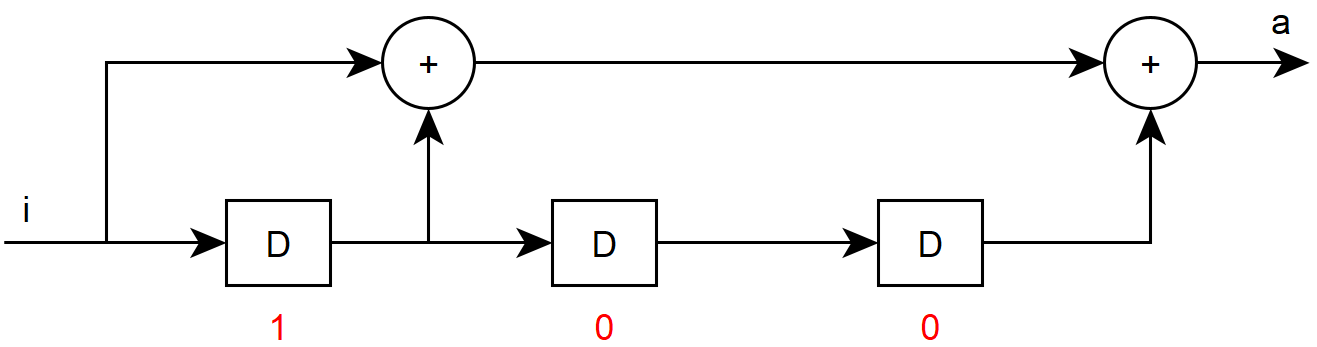
\includegraphics[width=7cm]{img/faltungscoder1in1out.PNG}

Impulsantort: $\displaystyle{
    g = 1 + 1D + 0D^2 + D^3 = 1 + D + D^3
}$

Generatorsequenz: $\displaystyle{\vec{g}^T =
    \begin{pmatrix}
        1 & 1 & 0 & 1
    \end{pmatrix}
}$

Von links nach rechts steht \textcolor{red}{$ (1 0 0) $} in den Speicherzellen und es wird $i = 1$ hineingeschrieben

$\displaystyle{
    \hookrightarrow \vec{d} = \begin{pmatrix}
        1\\
        0\\
        0
    \end{pmatrix}
}$

$\displaystyle{
    a = \begin{pmatrix}
        1 & 1 & 0 & 1
    \end{pmatrix}
    \cdot
    \begin{pmatrix}
        1\\
        1\\
        0\\
        0
    \end{pmatrix}
    = 0    
}$

\subsubsection{Mehrere Ausgänge}

Filter mit mehreren Ausgängen

$n$ Impulsantorten des Filters geben $n$ verschiedene Ausgänge

Generatorsequenz wird zu Generatormatrix mit $n$ Generatorsequenzen

$\displaystyle{
    \vec{a} = G^T \cdot
    \begin{pmatrix}
        i\\
        \vec{d}
    \end{pmatrix} =
    \begin{pmatrix}
        a^{(1)}\\
        a^{(2)}
    \end{pmatrix}
}$\;\;\;\;\;\;\;\;\;\;\;\;\;
$\displaystyle{
    G^T =
    \begin{pmatrix}
        \vec{g_1}^T\\
        \vec{g_2}^T
    \end{pmatrix}
}$

Ausgangssequenz: $a = a^{(1)}_1, a^{(2)}_1, a^{(1)}_2, a^{(2)}_2, ...$

\textbf{Beispiel}

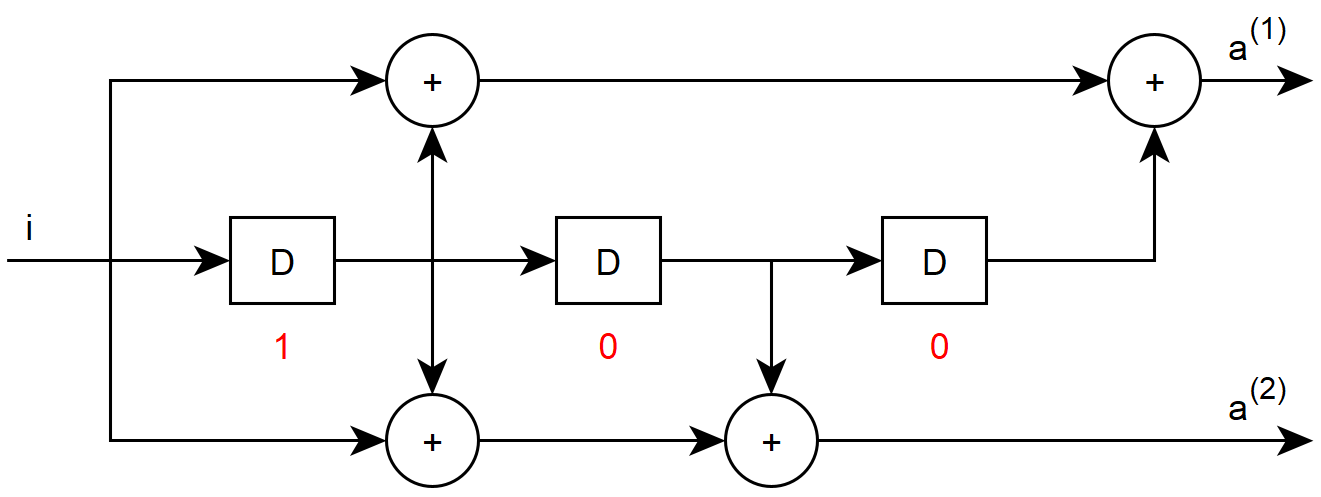
\includegraphics[width=7cm]{img/faltungscoder1in2out.PNG}

Im Speicher steht wieder von links nach rechts \textcolor{red}{$ (1 0 0) $} und es wird $i = 1$ hineingeschrieben

$\displaystyle{
    \vec{a} =
    \begin{pmatrix}
        1 & 1 & 0 & 1\\
        1 & 1 & 1 & 1
    \end{pmatrix}
    \cdot
    \begin{pmatrix}
        1\\
        1\\
        0\\
        0
    \end{pmatrix} =
    \begin{pmatrix}
        0\\
        0
    \end{pmatrix}
}$

\subsubsection{Mehrere Eingänge}

Mehrere Eingänge ($i^{(1)}, i^{(2)}$) um Coderate anzupassen

für jeden Ausgang gibt es jeweils $n$ Generatorsequenzen ($g_{ij}$)

$i$: Eingang\\
$j$: Ausgang

\textbf{Beispiel}

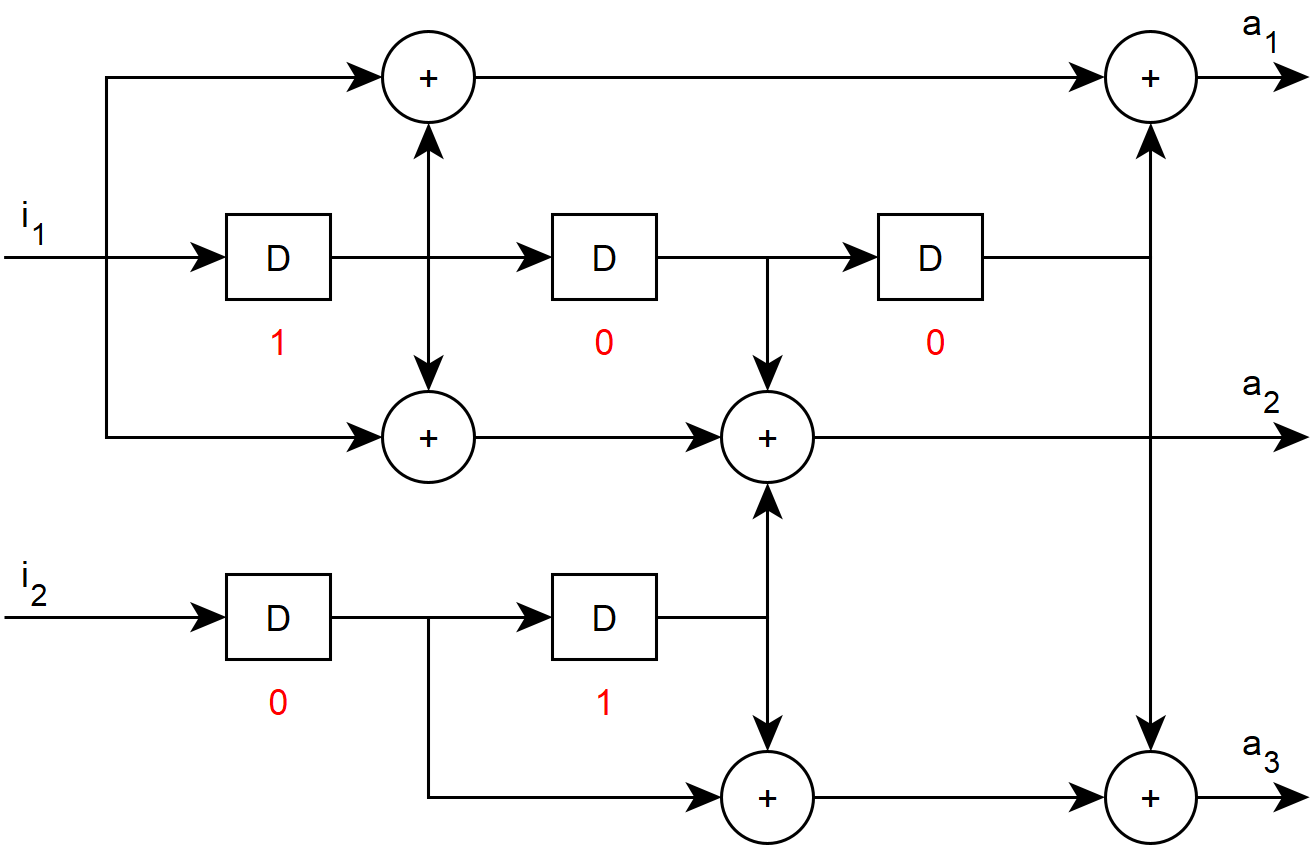
\includegraphics[width=7cm]{img/faltungscoder2in3out.PNG}

$\displaystyle{
    \vec{g_{11}}^T = \begin{pmatrix}
        1 & 1 & 0 & 1
    \end{pmatrix}
    \;\;\;\;\;\;\;
    \vec{g_{21}}^T = \begin{pmatrix}
        0 & 0 & 0 & 0
    \end{pmatrix}
}$

$\displaystyle{
    \vec{g_{12}}^T = \begin{pmatrix}
        1 & 1 & 1 & 1
    \end{pmatrix}
    \;\;\;\;\;\;\;
    \vec{g_{22}}^T = \begin{pmatrix}
        0 & 0 & 1 & 0
    \end{pmatrix}
}$

$\displaystyle{
    \vec{g_{13}}^T = \begin{pmatrix}
        0 & 0 & 0 & 1
    \end{pmatrix}
    \;\;\;\;\;\;\;
    \vec{g_{23}}^T = \begin{pmatrix}
        0 & 1 & 1 & 0
    \end{pmatrix}
}$
\\

Zusamenfassung in $G$

\begin{equation*}
    G = 
    \begin{tikzpicture}[baseline={-0.5ex},mymatrixenv]
        \matrix [mymatrix,inner sep=4pt] (m)  
        {
            1 & 0 & 1 & 0 & 0 & 0 & 1 & 0\\
            1 & 0 & 1 & 0 & 1 & 1 & 1 & 0\\
            0 & 0 & 0 & 1 & 0 & 1 & 1 & 0\\
        };
    
        % Braces
        \mymatrixbracebottom{2}{1}{$D^0$}
        \mymatrixbracebottom{4}{3}{$D^1$}
        \mymatrixbracebottom{6}{5}{$D^2$}
        \mymatrixbracebottom{8}{7}{$D^3$}
        \mymatrixbraceleft{1}{1}{Ausgang 1}
        \mymatrixbraceleft{2}{2}{Ausgang 2}
        \mymatrixbraceleft{3}{3}{Ausgang 3}
        \mymatrixbracetop{1}{1}{E1}
        \mymatrixbracetop{2}{2}{E2}
        \mymatrixbracetop{3}{3}{E1}
        \mymatrixbracetop{4}{4}{E2}
        \mymatrixbracetop{5}{5}{E1}
        \mymatrixbracetop{6}{6}{E2}
        \mymatrixbracetop{7}{7}{E1}
        \mymatrixbracetop{8}{8}{E2}
    \end{tikzpicture}
\end{equation*}

\subsection{Modifikationen}

\textbf{Punktierung}

Streichen bestimmmter Stellen aus dem Codewort

Punktierung über Punktierungsmatrix gegeben

Bsp.: für einen Coder mit 2 Ausgängen\\
\begin{equation*}
    G = 
    \begin{tikzpicture}[baseline={-0.5ex},mymatrixenv]
        \matrix [mymatrix,inner sep=4pt] (m)  
        {
            1 & 0\\
            1 & 1\\
        };
        % Braces
        \mymatrixbraceleft{1}{1}{Ausgang 1}
        \mymatrixbraceleft{2}{2}{Ausgang 2}
    \end{tikzpicture}
\end{equation*}

Ausgangssequenz $a$ punktieren durch bitweise AND mit der Matrixssequenz $p = (1\;1\;0\;1)$:\\

$a = \;\;1001\;0100\;1011\;1001\;0100$\\
$p = \;\;1101\;1101\;1101\;1101\;1101$

$a^* =  10x1\;01x0\;10x1\;10x1;01x0$

$x$: gestrichene Stelle, wird nicht übertragen (wird im Trellis immer als Fehler gewertet)

\textbf{Terminierung}

Endzustand des Coders bekannt, durch Anhängen von $z$ Nullen

$\hookrightarrow$ damit ist garantiert, dass im Coder am Ende nur Nullen stehen

\textbf{Tail-Biting}

Endzustand nach Codierung eines Informationswortes wird als Anfangszustand für eine erneute Codierung
verwendet (bei FIR-Filtern ist eine erste Codierung nicht notwendig, da der Endzustand nur von den letzten
$z$ Informationsbits abhängt)

$\hookrightarrow$ damit ist der Anfangszustand identisch mit Endzustand

$\hookrightarrow$ der Decoder decodiert und kennt mit großer Sicherheit den Anfangszustand und damit auch den
Endzustand

\subsection{Decodierung}

Mit Viterbi-Algorithmus

Konstruktion eines Zustandsgraphen für den Coder

Aus Zustandgraph wird Trellis-Diagramm erstellt

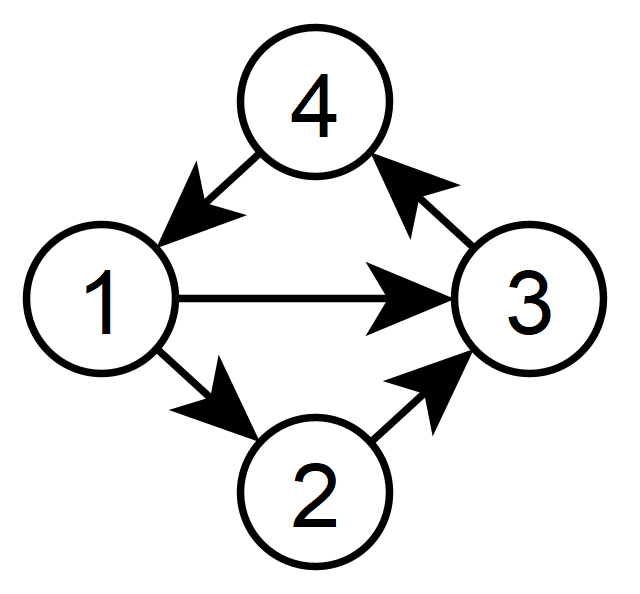
\includegraphics[width=3cm]{img/zustandsgraph.PNG}
\;\;\;\;
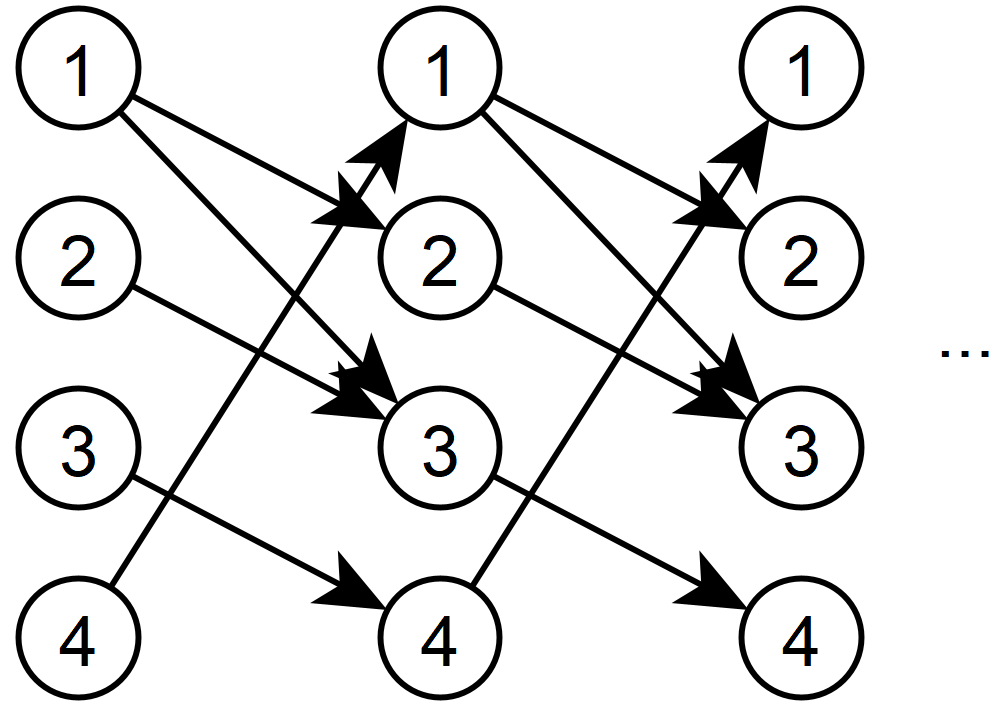
\includegraphics[width=4cm]{img/trellis.PNG}

gesucht: Informationsfolge, welche in den Coder geschickt wurde

Metrik: Anzahl der übereinstimmenden Ausgangsbits

Pfad mit höchster Übereinstimmung wird genommen

\underline{Außer}:
\begin{itemize}
    \item bei Terminierung: Endzustand 0
    \item bei Tail-Biting: Endzustand = Anfangszustand
\end{itemize}

	\newpage
	\appendix
	\appendix

\section{Hilfreiches}

\subsection{Inverse in Galois-Feldern}

\textbf{Additive Inverse}

gegeben: $-3$ in $GF(5)$

gesucht: additive Inverse

bedeutet: $3 + x \mod 5 = n = 0$

$x = 2$ , da $3 + 2 = 5$ und $5 \mod 5 = 0$

daher: $-3 = 2$

$n$: neutrales Element der Addition ($=0$)

\underline{oder}: mit Tabelle

gegebene Zahl als Index behandeln, passenden Wert raussuchen

\begin{tabular}{ c | c | c | c | c | c | c | c | c | c | c | c | }
    Index & -3 & -2 & -1 & 0 & 1 & 2 & 3 & 4 & 5 & 6\\
    \hline
    Wert  & 2  &  3 &  4  & 0 & 1 & 2 & 3 & 4 & 0 & 1
\end{tabular}

\textbf{Multiplikative/modulare Inverse}

gegeben: $2^{-1}$ in $GF(7)$

gesucht: multiplikative Inverse

bedeutet: $2^{1} \cdot x \mod 7 = n = 1$

$x = 4$ , da $2^{1} \cdot 4 = 8$ und $8 \mod 7 = 1$

daher: $2^{-1} = 4$

\underline{oder}: mit Logarithmentafel

gegebene Potenz als Index behandeln, passenden Wert raussuchen

\begin{tabular}{ c | c | c | c | c | c | c | c | c | c | c | c | }
    Index  & -3 & -2 & -1 & 0 & 1 & 2 & 3 & 4 & 5 & 6\\
    \hline
    Wert   &  1 &  2 &  4 & 1 & 2 & 4 & 1 & 2 & 4 & 1
\end{tabular}

\subsection{ABC/PQ-Formel}

\textbf{ABC/ PQ-Formel}

ABC: $ax^2 + bx + c = 0$

$\displaystyle{
    x_{1,2} = \frac{-b \pm \sqrt{ b^2 - 4ac }}{2a}
}$

PQ: $x^2 + px + q$

$\displaystyle{
    x_{1,2} = -\frac{p}{2} \pm \sqrt{\left(\frac{p}{2}\right)^2 - q}
}$

\section{Polynome}

\subsection{Polynommultiplikation}

\subsection{Polynomdivision}

\section{Lineare Algebra}

\textbf{Matrix-Multiplikation}

$\displaystyle{
    A \cdot B = 
    \begin{pmatrix}
        a & b\\
        c & d\\
        e & f
    \end{pmatrix}_{\color{red} 3 , \color{green} 2 }
    \begin{pmatrix}
        g & h\\
        i & j
    \end{pmatrix}_{\color{green} 2, \color{blue} 2}
    = 
    \begin{pmatrix}
        a g + b i & a h + b j\\
        c g + d i & c h + d j\\
        e g + f i & e h + f j
    \end{pmatrix}_{\color{red} 3, \color{blue} 2}
}$

$\displaystyle{
    \vec{v} \cdot \vec{w}^T = 
    \begin{pmatrix}
        a \\
        b\\
        c
    \end{pmatrix}
    \cdot
    \begin{pmatrix}
        d & e & f
    \end{pmatrix}
    = 
    \begin{pmatrix}
        a \cdot d & a \cdot e & a \cdot f\\
        b \cdot d & b \cdot e & b \cdot f\\
        c \cdot d & c \cdot e & c \cdot f
    \end{pmatrix}
}$

Skalarprodukt:

$\displaystyle{
    \vec{v}^T \cdot \vec{w} = 
    \begin{pmatrix}
        a & b & c
    \end{pmatrix}
    \cdot
    \begin{pmatrix}
        d\\
        e\\
        f
    \end{pmatrix}
    = a \cdot d + b \cdot e + c \cdot f
}$

bei komplexen Vektoren:
$\displaystyle{
    \vec{v}^H \cdot \vec{w}
}$

\textbf{Transponieren}

Zeilen werden Spalten, Spalten werden Zeilen

$\displaystyle{
    A^T =
    \begin{pmatrix}
        a & b & c\\
        d & e & f
    \end{pmatrix}^T
    =
    \begin{pmatrix}
        a & d\\
        b & e\\
        c & f
    \end{pmatrix}
}$

\textbf{Invertieren}

für 2x2-Matrizen:

$\displaystyle{
    A^{-1} =
    \begin{pmatrix}
        a & b\\
        c & d
    \end{pmatrix}^{-1}
    = \frac{1}{ad - bc}
    \begin{pmatrix}
        d & -c\\
        -b & a
    \end{pmatrix}
}$

\textbf{Diagonale Matrix}

$\displaystyle{
    \begin{pmatrix}
        1 & 0 & 0\\
        0 & -5 & 0\\
        0 & 0 & 3
    \end{pmatrix}
}$

Spalten der Matrix sind Eigenvektoren

1; -5; 3 sind die Eigenwerte der Eigenvektoren

\textbf{Hermitesche Matrix}

nur für quadratische Matrizen

$\displaystyle{
    A = A^H = (A^*)^T =
    \begin{pmatrix}
        1 & 5 - j & 3j\\
        5 + j & 2 & 3 - 2j\\
        -3j & 3 + 2j & 3 +4j
    \end{pmatrix}
}$

Eigenvektoren von hermiteschen Matrizen sind orthogonal

\textbf{Unitäre Matrix}

$\displaystyle{
    A \cdot A^H = k \cdot I
}$

$k$: Skalierungsfaktor (bei skaliert unitären Matrizen)

\textbf{Toeplitz-Struktur}

Eine Matrix hat Toeplitz-Struktur, wenn alle Diagonalen parallel zur Hauptdiagonalen, die gleichen Elemente enthalten:

$\displaystyle{
    T =
    \begin{pmatrix}
        0 & -2 & -5 & -3\\
        1 & 0 & -2 & -5 \\
        2 & 1 & 0 & -2  \\
        3 & 2 & 1 & 0
    \end{pmatrix}
}$
 
Hermitesche Toeplitz-Matrizen sind positiv oder negativ definit, abhängig vom Vorzeichen der
Elemente auf der Hauptdiagonalen

\textbf{Vandermonde-Matrix}

Spalten: Indezes gleich\\
Zeilen: Potenzen gleich

$\displaystyle{
    S =
    \begin{pmatrix}
        1 & 1 & ... & 1\\
        x_0^1 & x_1^1 & ... & x_{N-1}^1\\
        x_0^2 & x_1^2 & ... & x_{N-1}^2\\
        ... & ... & ... & ...\\
        x_0^{N-1} & x_1^{N-1} & ... & x_{N-1}^{N-1}
    \end{pmatrix}
}$

\textbf{Determinante}

nur für quadratische Matrizen

für $2 \times 2$-Matrix:

$\displaystyle{
    det(A) = det\left[
        \begin{pmatrix}
            a & b\\
            c & d
        \end{pmatrix}
    \right] = 
    a \cdot d - b\cdot c
}$

für $3 \times 3$-Matrix:

$\displaystyle{
    det(C) = det\left[
        \begin{pmatrix}
            a & b & c\\
            d & e & f\\
            g & h & i
        \end{pmatrix}
    \right]
}$

$\displaystyle{
    = a \cdot det\left[ \begin{pmatrix}
        e & f\\
        h & i
        \end{pmatrix} \right]
    - b \cdot det\left[ \begin{pmatrix}
        d & f\\
        g & i
        \end{pmatrix} \right]
    + c \cdot det\left[ \begin{pmatrix}
        d & e\\
        g & h
        \end{pmatrix} \right]
}$

\textbf{Rang einer Matrix}

Eine Matrix hat vollen Rang, wenn die Determinante ungleich 0 ist

Ist die Determinante gleich 0, ist die Matrix/das Gleichungssystem überbestimmt

\textbf{Eigenvektoren/ Eigenwerte}

Eigenvektoren einer Matrix werden bei einer Matrixtransformation nur in ihrer Länge geändert,
nicht in ihrer Richtung

Faktor, um den ein Eigenvektor gedehnt oder gestaucht wird, ist der zum Eigenvektor zugehöriger
Eigenwert $\lambda$

$\displaystyle{
    A \vec{v} = \lambda \vec{v}
}$

$\displaystyle{
    (A - \lambda I) \vec{v} = \vec{0}
}$

$A$: Matrix\\
$\vec{v}$: Eigenvektor\\
$\lambda$: Eigenwert(e)\\
$I$: Einheitsmatrix

Eigenwerte von positiv (oder negativ) definiten Matrix sind immer positiv (oder negativ)


\section{Digitale Signalverarbeitung}

\textbf{Diskretisierung und Fensterung}

Diskretisierung \laplace \; Periodische Fortsetzung\\
Diskretisierung \Laplace \; Periodische Fortsetzung\\
Begrenzung $\rightarrow$ Leck-Effekt

\textbf{Fourier-Transformation (kontinuierlich)}

$\displaystyle{
    X(f) = \int_{-\infty}^{\infty} x(t) \cdot e^{-j2\pi ft} \, dt
}$

\textbf{DFT}

$\displaystyle{
    X(n) = \sum_{k=0}^{N-1} x(k) \cdot e^{-j2\pi \frac{nk}{N}}
}$

$n$: Frequenzindex\\
$k$: Zeitindex

\textbf{Auflösung DFT}

$\displaystyle{
    \Delta f = \frac{f_a}{N} = \frac{1}{t_a \cdot N} = \frac{1}{\Delta t}
}$

$\Delta f$: spektrale Auflösung\\
$f_a$: Abtastfrequenz\\
$t_a$: Abtastrate\\
$N$: Anzahl Abtastwerte\\
$\Delta t$: Messdauer

\textbf{Fensterung}

Fensterung im Zeitbereich $\rightarrow$ Multiplikation mit Fensterfunktion \laplace \; Faltung mit zur Fensterfunktion zugehörigem Spektrum

\textbf{Dirichlet-Kern}

abgetastete Rechteckfunktion \laplace \; Dirichlet-Kern

Definition der Dirichlet-Kerns der Länge $N+1$:

$\displaystyle{
    D(x) = \sum_{n=-\frac{N}{2}}^{\frac{N}{2}} e^{jnx} =
    \frac{\sin\left( \left( \frac{N + 1}{2} \right) x \right)}{\sin\left( \frac{x}{2} \right)}
}$

$x = 2\pi fT_a$

Bsp: 11:

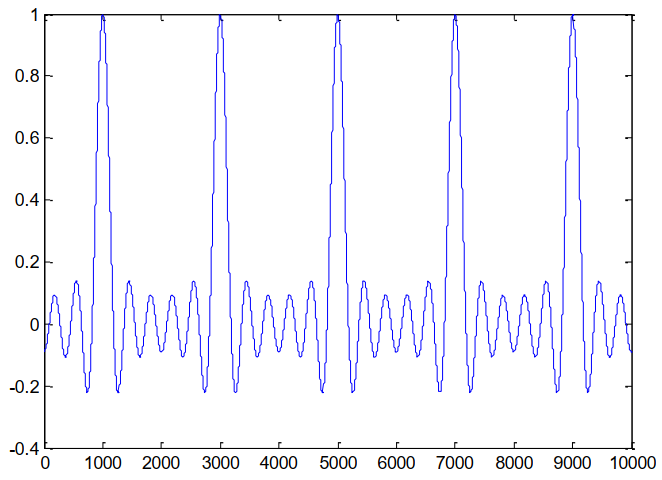
\includegraphics[width=6cm]{img/dirichlet-kern.png}

Eigenschaften:

Hauptwert hat Höhe $N+1$\\
Nullstellen, bei $\displaystyle{
    f = \frac{f_a}{N+1} \cdot k
}$ für
$\displaystyle{
    k \in \mathbf{N}
}$\\
Hauptwert periodisch mit $f_a$

\textbf{z-Transformation}

$\displaystyle{
    z = e^{j2\pi \frac{f}{f_a}}
}$

$\displaystyle{
    H(f) = H(z) \bigg \vert _{z=e^{j2\pi \frac{f}{f_a}}}
}$

\textbf{Reiner FIR-Filter}

kanonische Form

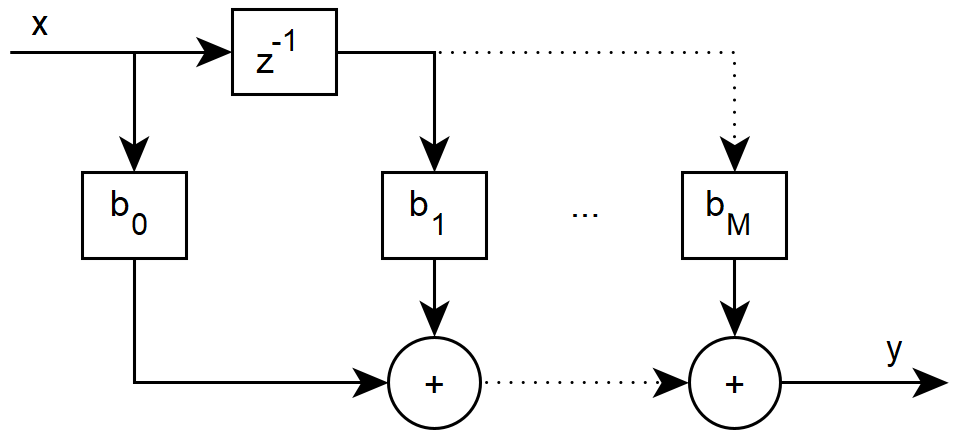
\includegraphics[width=6cm]{img/fir.png}

$\displaystyle{
    H(z) = \frac{Y(z)}{X(z)} = b_0 + b_1 \cdot z^{-1} + ... + b_M \cdot z^{-M}
}$

$\displaystyle{
    y(t) = b_0 \cdot x(t) + b_1 \cdot x(t-1) + ... + b_M \cdot x(t-M)
}$

\textbf{Reiner IIR-Filter}

kanonische Form

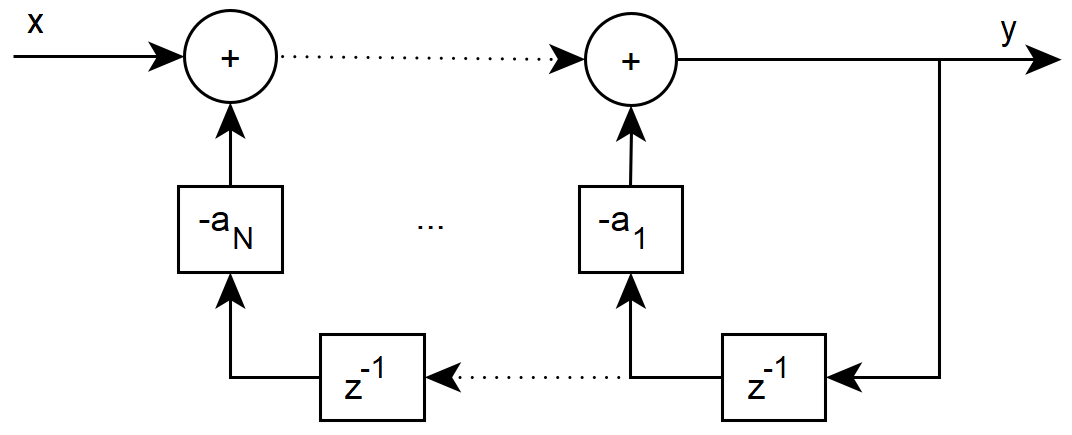
\includegraphics[width=6.5cm]{img/iir.png}

$\displaystyle{
    H(z) = \frac{1}{1 + a_1 \cdot z^{-1} + ... + a_N \cdot z^{-N}}
}$

$\displaystyle{
    y(t) = x(t) - a_1 \cdot y(t-1) - ... - a_n \cdot y(t-N)
}$
	
	\cleardoublepage
	
	%% Quellenverzeichnis
	%%\printbibliography[title=Quellenverzeichnis]
	%%\addcontentsline{toc}{section}{Quellenverzeichnis}

%%%%%%%%%%%%%%
\end{document}
%%%%%%%%%%%%%%
